\documentclass[a4paper, 14pt, titlepage]{extarticle}
  \usepackage{cmap}
  \usepackage[hidelinks,pdftex,unicode]{hyperref}
  \usepackage{mathtext} % для кириллицы в формулах
  \usepackage[T2A]{fontenc}
  \usepackage[utf8]{inputenc}
  \usepackage[english,russian]{babel}
  \usepackage{indentfirst}
  \usepackage{cite}
  \usepackage{amsmath} % для \eqref
  \usepackage{color} % пока только для TODO:
  \usepackage[pdftex]{graphicx}
  \usepackage{subfig}
  \graphicspath{{../img/}{../../img/}}
  \frenchspacing

  \DeclareSymbolFont{T2Aletters}{T2A}{cmr}{m}{it} % кириллица в формулах курсивом

  \addto\captionsrussian{
    \renewcommand\contentsname{Содержание}
    \let\oldrefname\refname
    \renewcommand\refname{\addcontentsline{toc}{section}{\oldrefname}\oldrefname}
  }

  \newcommand{\underscore}[1]{\hbox to#1{\hrulefill}}
  \newcommand{\todo}[1]{\textbf{\textcolor{red}{TODO: #1}}}
  \newcommand{\note}[1]{\textit{Примечание: #1}}
  \newcommand{\eng}[1]{{\English #1}}

  % вставка картинки: \figure[params]{file}{описание}
  \newcommand{\includefigure}[3][]{
    \begin{figure}[!htb]
      \center{\includegraphics[#1]{#2}}
      \caption{#3} \label{fig:#2}
    \end{figure}
  }

  \newcommand{\vect}[1]{\vec{#1}} % единое выделение векторов (стрелкой)
  \newcommand{\matx}[1]{\mathbf{#1}} % единое выделение матриц (полужирным)
  \newcommand{\transposed}{\top} % единый знак транспонирования (U+22A4 down tack)

  % поля и размер текста
  \textwidth=17cm
  \oddsidemargin=0pt
  \topmargin=0pt
  \headheight=0pt
  \headsep=0pt
  \textheight=24cm
  \linespread{1.3}

  % русские буквы для списков и частей рисунка
  \renewcommand{\theenumii}{(\asbuk{enumii})}
  \renewcommand{\labelenumii}{\asbuk{enumii})}
  \renewcommand{\thesubfigure}{\asbuk{subfigure}}

  \let\oldsection\section
  \renewcommand{\section}{\newpage\oldsection}

  \setcounter{tocdepth}{2} % глубина оглавления

  \bibliographystyle{gost780u}

  \hyphenation{англ} % убрать перенос в этом сокращении

  \author{И.\,А.\,Новиков, кафедра АФТИ ФФ НГУ, гр.\,7305}
  \title{Система моделирования деформаций неупругих тел в реальном времени}

\begin{document}

%----------------------- титульный лист ------------------------

  \thispagestyle{empty}
  \begin {center}
  МИНИСТЕРСТВО ОБРАЗОВАНИЯ И НАУКИ РОССИЙСКОЙ ФЕДЕРАЦИИ

  \vspace{0.3cm}

  Новосибирский государственный университет

  \vspace{0.3cm}

  Физический факультет

  Кафедра автоматизации физико-технических исследований

  \vspace {5cm}

  Апрельский отчёт

  \vspace {1cm}

  Новиков Иван Александрович

  \vspace {0.5cm}

  \textbf{СИСТЕМА МОДЕЛИРОВАНИЯ ДЕФОРМАЦИЙ НЕУПРУГИХ ТЕЛ В РЕАЛЬНОМ ВРЕМЕНИ}

  \vspace {2cm}

  \begin{flushright}

    Научный руководитель

    Д.\,А.\,Гладкий

  \end{flushright}

  \vspace {5cm}

  Новосибирск, 2011~г.
  \end {center}

%------------------------- содержание -------------------------

  \tableofcontents
  \newpage

%-------------------------- введение --------------------------
  \section{Введение}

    Приложения виртуальной реальности становятся чрезвычайно рас\-прос\-тра\-нён\-ны\-ми в~наши~дни.  Два
    основных их типа~--- это компьютерные игры и~обучающие симуляторы (тренажёры). Несмотря на
    различные применения, эти два типа приложений имеют много общего, поскольку в~обоих случаях
    требуется создать иллюзию присутствия у~пользователя. Для~этого необходимо как генерировать
    фотореалистичные изображения, так и правдоподобно моделировать физику взаимодействия объектов
    виртуального мира: их движение, столкновения, деформации и~разрушение.

    Моделирование деформаций объектов является актуальной задачей, поскольку помимо приложений
    виртуальной реальности оно находит применение в~системах автоматизированного проектирования, а~также используется
    при~создании спецэффектов к~фильмам. В зависимости от поставленной задачи применяются различные
    подходы. А~именно, в~системах автоматизированного проектирования требуется
    максимальная точность расчётов, в~то~время как в~фильмах и приложениях виртуальной реальности
    требуется лишь визуальная правдоподобность. При~этом, если расчёты для САПР и~спецэффектов могут
    выполняться длительное время, то в~интерактивных приложениях расчёт одного шага вычислений должен
    происходить не~дольше, чем за~промежуток между кадрами, чтобы обеспечивать плавную анимацию
    и чтобы отсутствовала задержка между воздействием на объект и его деформацией.

    Жёсткое требование быстродействия в приложениях реального времени не~только вынуждает
    использовать упрощённые физические модели деформации тела, менее точные, чем используемые
    в~инженерных расчётах, но и накладывают существенные ограничения на способ представления
    моделируемого объекта. Чаще всего он задаётся дискретным образом: в~виде сетки, решётки или
    несвязанного набора точек, причём время расчётов напрямую (как~правило, линейно
    \cite{mueller-meshless}) зависит от количества точек в таком представлении. Для отображения
    объектов обычно используют высоко детализированные сетки, содержащие вплоть до нескольких
    сотен тысяч и даже миллионов точек. Это значительно превышает максимальное допустимое число точек для~большинства
    алгоритмов \cite{mueller-stable, mueller-meshless, chang-crash} при расчётах в~реальном времени на
    современных настольных компьютерах и компьютерах, используемых в тренажёрах. Из-за этого
    невозможно использовать одно и~то~же представление объекта и для моделирования, и для
    отображения.

  \section{Описание предметной области}\label{sec:domain}

    Существуют различные подходы к~моделированию деформаций в~реальном времени. В простейшем случае
    ограничения на~быстродействие алгоритма обходятся за счёт использования предварительно рассчитанных
    деформированных состояний для~некоторого конечного набора возможных ударов по~объекту, одно из которых
    (или~интерполяция между несколькими ближайшими) выбирается в~зависимости от~того, к~какому
    из~этих ударов ближе всего произошедший. В~этом случае допускается использование достаточно сложных
    для~вычисления алгоритмов, таких~как система масс и~пружин (англ. \eng{mass-spring system})
    с~большим разрешением или~метод конечных элементов (англ. \eng{finite elements method, FEM}).
    Однако, при ударе, отличающемся от~заранее рассчитанного, или в~случае сложной комбинации ударов
    моделируемые деформации будут выглядеть не реалистично \cite[с.~1064]{chang-crash}. Кроме того, значительное время, требуемое
    для предварительных расчётов после каждого изменения объекта, прежде чем он может быть загружен
    в приложение для тестирования, создаёт неудобства при разработке приложения. Поэтому наибольший
    интерес представляют решения, в которых моделирование деформаций происходит во время исполнения.

    Одной из~простейших моделей деформируемого тела является упоминавшаяся выше система масс
    и~пружин, в~которой тело представляется в~виде пространственной (как~правило, регулярной и
    кубической) решётки из~материальных точек, связанных между~собой пружинами, при~изменении длины
    прикладывающими к~своим концам силу согласно закону Гука. Будучи очень простой в~реализации,
    такая модель, тем не менее, имеет определённые недостатки. Она моделирует поведение объекта не
    очень точно, причём оно сильно зависит от формы решётки и расположения пружин в ней \cite[с.~8]{mueller-physmodels}.
    Другим недостатком является то, что возбуждение, приложенное локально, распространяется по
    объекту постепенно, перемещаясь на один шаг решётки за шаг алгоритма \cite[с.~232]{parent-animation}.
    Кроме~того, требуется выполнять дополнительную работу по конвертации представления объекта,
    используемого для его отображения (чаще всего это сетка из треугольников), в~регулярную решётку
    и~подбору значений коэффициента упругости пружин так, чтобы добиться требуемых свойств
    моделируемого материала.

    Принципиально другой подход реализуется в моделях, использующих метод конечных элементов, широко
    используемый в~инженерных расчётах. При таком подходе
    непрерывные характеристики деформируемого тела вычисляются путём интерполяции их~значений
    на~элементах конечного размера. Разумеется, использовать в чистом виде этот метод
    в приложениях реального времени невозможно, поскольку инженерные расчёты производятся в
    течение нескольких часов и даже суток. Однако, существуют модели, предлагающие различные упрощения этих
    методов, которые допускают вычисление в реальном времени, как, например в \cite{mueller-stable}.
    Деформации при этом моделируются намного точнее, чем в случае системы масс и пружин, но даже
    упрощённый алгоритм требует больше времени для вычислений. % TODO циферки

    Отдельно стоят так~называемые геометрические алгоритмы, в~которых напрямую не~моделируются
    физические законы. Как~правило, объект представляется в~виде системы частиц, движение каждой из
    которых сначала интегрируется независимо от~остальных, а~следующим шагом на объект в~целом
    накладываются различные физически мотивированные ограничения (сохранение формы, объёма, импульса
    и~т.п.), обеспечивающие в итоге правдоподобные деформации. Такие методы обладают хорошим
    быстродействием и могут вычисляться параллельно, при этом обладая большей устойчивостью и
    простотой в конфигурации, чем системы масс и пружин. Пример такого метода описывается в \cite{mueller-meshless}.

  \section{Постановка задачи}\label{sec:task}

    Целью работы является разработка системы моделирования деформаций объектов для применения в
    приложениях виртуальной реальности: в компьютерных играх и обучающих тренажёрах.
    К~системе предъявляются следующие требования.

    Необходимо использовать сетки из треугольников в качестве внутреннего представления, либо
    предоставить возможность конвертации, поскольку в приложениях виртуальной реальности отображаемые объекты
    чаще всего представляются именно в таком формате. Это связано с~тем, что треугольник является
    основным геометрическим примитивом для графических процессоров. % TODO пруф

    Система должна иметь достаточное быстродействие, чтобы обеспечивать моделирование в~реальном
    времени. Известно, что для комфорта пользователя и ощущения им реалистичности моделируемого мира
    приложение виртуальной реальности должно обеспечивать кадровую частоту около 30 кадров в секунду
    и выше \cite{claypool-framerate}. Следовательно, все расчёты, необходимые для получения
    следующего кадра, в таком приложения должны занимать не более 33 мс. Поскольку расчёт глобального
    движения и трёхмерной графики обычно является более приоритетной задачей, на вычисление
    деформаций отводится небольшая часть этого времени, около 3-5 мс. Чтобы такое быстрое
    моделирование было возможно даже для~объектов, заданных сеткой с~большим числом вершин,
    должна иметься возможность использовать при~моделировании менее детализированное представление
    объекта, а~отображаемую сетку более высокого разрешения обновлять так, чтобы она повторяла
    рассчитанные деформации. При~этом важно предусмотреть некоторое сглаживание смещений точек
    отображаемого объекта, иначе в~их~движении можно будет проследить форму низко детализированного
    представления.

    Для эффективного использования вычислительной мощности многоядерных центральных процессоров,
    получающих в наши дни всё большее распространение, необходимо, чтобы вычисления могли
    выполняться параллельно.

    Кроме~того, предварительно рассчитанные деформированные состояния не~должны использоваться,
    поскольку, как было объяснено в разделе~\ref{sec:domain}, такой подход негативно сказывается на реалистичности
    моделирования и создаёт неудобства при разработке приложения.

    Наконец, интерфейс, предоставляемый системой, не~должен создавать трудностей при~интеграции
    системы в~приложения виртуальной реальности. Основные критерии, которым необходимо следовать,
    описаны в~\cite{gems-middleware} и~включают, в~частности, конфигурируемые обработку ошибок,
    журналирование и~выделение памяти, а также отказ от~прямого доступа к~файловой системе в~пользу
    работы с~буферами в~оперативной памяти.

    Для достижения цели необходимо решить следующие задачи.
    \begin{enumerate}
      \item Разработать и~реализовать алгоритм моделирования в реальном времени деформаций
        не\-у\-пру\-гих тел, содержащих недеформируемые части;
      \item Предоставить интерфейс для~двустороннего взаимодействия с~приложением, в~которое будет
        встроена система, включающий:
        \begin{enumerate}
          \item конвертацию представления объекта, используемого в приложении, во внутреннее представление;
          \item получение извне информации о~столкновениях объекта и~приложенных к~нему силах;
          \item уведомление о произошедших событиях, характеризующих сильные локальные деформации;
          \item обновление отображаемой сетки.
        \end{enumerate}
      \item Предусмотреть в~алгоритме возможность использования параллельных вычислений.
    \end{enumerate}

  \section{Система моделирования деформаций}
    \subsection{Архитектура системы}

      Система реализуется в~виде модуля, который может быть встроен в~приложение виртуальной
      реальности: статической либо динамической библиотеки, написанной на языке C++. Выбор языка
      обоснован компромиссом между быстродействием и удобством разработки и интеграции, которые
      обеспечивает использование объектно-ориентированной парадигмы. Не менее важно, что большинство
      компьютерных игр и~других приложений виртуальной реальности написаны именно на этом языке
      программирования, поэтому требование лёгкости интеграции также влияет на выбор в~пользу C++.

      В~системе выделяются следующие подсистемы.
      \begin{enumerate}
        \item Ядро системы, обеспечивающее собственно моделирование.
        \item Подсистема математических расчётов.
        \item Подсистема журналирования и~обработки ошибок.
      \end{enumerate}

      \subsubsection{Ядро системы}\label{sssec:core}

        Ядро системы реализует класс <<деформируемый физический объект>>. Он инициализируется
        начальной конфигурацией объекта и~предоставляет интерфейс для совершения с~ним следующих действий.
        \begin{enumerate}
          \item Задание недеформируемых частей объекта (при наличии таковых).
          \item Задание приложенных сил и~произошедших столкновений.
          \item Определение реакции на события, происходящие при~деформации объекта.
          \item Моделирование процесса деформаций для~заданного промежутка времени.
          \item Обновление формы отображаемой сетки.
        \end{enumerate}

        Таким образом, для~обеспечения перечисленной функциональности система также реализует следующие классы.
        \begin{enumerate}
          \item Сила, приложенная к~объекту.
          \item Реакция на событие.
          \item Область в~трёхмерном пространстве.
          \item Описатель формата отображаемой сетки.
        \end{enumerate}

      \subsubsection{Подсистема математических расчётов}

        Подсистема математических расчётов реализует необходимые для~расчёта деформаций математические объекты
        и~функции. Их набор зависит от выбранного алгоритма и будет описан далее, в п.~\ref{sssec:math}.

      \subsubsection{Подсистема журналирования и~обработки ошибок}

        Данная подсистема обеспечивает обработку ошибок и~предупреждений, возникающих в~процессе
        работы системы, а~также запись в журнал. В приложении, использующем систему, может
        быть реализована своя политика журналирования и обработки ошибок. Для удобства интеграции
        стандартные действия, выполняемые в ответ на каждое из этих событий, можно переопределить
        в~соответствии с политикой приложения.

      \subsection{Основной алгоритм}\label{ssec:basic_algorithm}

      В разделе~\ref{sec:domain} были рассмотрены различные подходы к моделированию деформаций.
      В~частности, было показано, что системы масс и пружин не обеспечивают требуемого качества
      моделирования и требуют дополнительного преобразования формата объекта, а упрощённый метод конечных элементов
      хоть и моделирует деформации очень реалистично, но имеет значительно худшее быстродействие.
      Геометрические же алгоритмы работают очень быстро, но нужно правильно выбрать используемые в
      них ограничения и подобрать параметры, чтобы моделирование было реалистичным в каждом
      конкретном случае. В данной работе за основу алгоритма моделирования взят геометрический
      алгоритм, предложенный в~\cite{mueller-meshless}. Затем он адаптирован для текущей задачи.

      \subsubsection{Исходный алгоритм}

        \paragraph{Входные данные и результат.} Объект представляется в~виде набора точек,
        сгруппированных в~перекрывающиеся множества, называемые кластерами
        (информация о~связях между вершинами, то~есть об~образуемых ими полигонах, не требуется).
        На~вход алгоритма поступает заданный таким образом объект, а так же информация о~приложенных
        силах. Задаётся величина шага по времени. Результатом выполнения одной итерации алгоритма
        являются позиции точек, задающих объект, в следующий момент времени.

        \paragraph{Общая схема алгоритма.} Скорости и позиции этих точек интегрируются независимо
        друг от друга, для чего используется явная схеме Эйлера. Затем над каждым кластером
        производится операция сопоставления формы: вычисляется новое положение центра масс кластера
        $\vect{x}_{ц.м.}$ и оптимальное линейное преобразование $\matx A$, действие которого
        переводит исходную форму кластера в~наиболее близкую к~текущей форме. В качестве критерия
        оптимальности используется сумма квадратов отклонений текущий позиций точек от начальных. Позиции
        вершин в кластере, подвергнутые оптимальному линейному преобразованию и смещению центра масс
        $\vect{g}_i = \matx{A} (\vect{x}^0_i - \vect{x}^0_{ц.м.}) + \vect{x}_{ц.м.}$,
        называются целевыми позициями. Здесь $\vect{x}^0_i$~--- исходная позиция вершины, а
        $\vect{x}^0_{ц.м.}$~--- исходный центр масс кластера. Для каждой вершины, исходя из величины
        отклонения текущей позиции от~целевой, рассчитывается поправка к~скорости, корректирующая
        это отклонение. Если вершина входит одновременно в~несколько кластеров, то~есть находится
        в~зоне их перекрытия, корректирующие поправки от~каждого из~кластеров усредняются, что
        обеспечивает целостность объекта: за~счёт этого кластеры, обрабатываемые независимо,
        не~отделяются друг от~друга.

        \paragraph{Остаточная деформация.} Для моделирования неупругости остаточная деформация
        каждого кластера сохраняется в~форме линейного преобразования $\matx{S}^{ост}$, то~есть
        матрицы $3 \times 3$. Изначально она единичная, а~изменение происходит, лишь когда мера
        текущей деформации превышает заданную пороговую величину. В~качестве такой меры может быть
        использована $ \|\matx S - \matx E\|_2 $, где $\matx S$~--- симметричная компонента $\matx
        A$, $\matx E$~--- единичная матрица, норма Фробениуса $\|\matx M\|_2 = \sqrt{\sum_{i, j} |m_{ij}|^2}$.
        Симметричная матрица $\matx S$ получается при полярном разложении матрицы $\matx A$:
        \begin{equation}\label{eq:polar_decomposition}
          \matx A = \matx R \matx S,
        \end{equation}
        где $\matx R$~--- ортогональная матрица. Остаточная деформация учитывается затем при
        сопоставлении формы и расчёте целевых позиций. А именно, исходные позиции перед сравнением
        с текущими при сопоставлении формы, преобразуются матрицей $\matx{S}^{ост}$. Таким
        образом, сопоставление происходит не с~исходной, а с деформированной формой. Формула для
        расчёта целевых позиций принимает следующий вид:
        \begin{equation}\label{eq:goal_pos}
          \vect{g}_i = \matx{A} \matx{S}^{ост} (\vect{x}^0_i - \vect{x}^0_{ц.м.}) + \vect{x}_{ц.м.}.
        \end{equation}

      \subsubsection{Предлагаемые изменения в алгоритме}\label{sssec:proposed_changes}

        В~исходный алгоритм вносятся изменения, адаптирующие его к~условиям данной
        задачи. Во-первых, моделирование неупругих тел требует демпфирования возникающих колебаний.
        Во-вторых, система отвечает только за~моделирование деформаций, а глобальное движение и
        определение столкновений рассчитываются отдельно приложением, в~которое встроена система.
        Поэтому расчёт деформаций необходимо производить в~локальных координатах~---
        в~неинерциальной системе отсчёта, связанной с центром масс объекта, в которой он не
        движется и не вращается. Далее для краткости она называется системой центра масс.

        \paragraph{Демпфирование.} Чтобы моделируемое поведение неупругого тела выглядело правдоподобным,
        нужно, чтобы затухали только колебания, а глобальное движение тела сохраняло свои характеристики.
        Для этого используется способ, описанный в~\cite[с.~5]{mueller-position-dynamics}. Сначала выделяется
        движение тела как~целого~--- вычисляются скорость центра масс $\vect{v}_{ц.м.}$ и угловая
        скорость $\vect{\omega}$. Для этого рассчитываются центр масс
        $\vect{x}_{ц.м.}$ и тензор инерции $\matx I$ (матрица $3 \times 3$):
        \begin{eqnarray*}
          \vect{x}_{ц.м.} & = & \frac{\sum_i m_i \vect{x_i}}{\sum_i m_i},\\
          \vect{r}_i      & = & \vect{x}_i - \vect{x}_{ц.м.},\\
          \matx{I}        & = & \sum_i m_i ( |\vect{r}_i|^2 \matx E - \vect{r}_i \vect{r}_i^\transposed),\\
        \end{eqnarray*}
        где $\matx E$~--- единичная матрица $3 \times 3$. Затем вычисляются
        \begin{eqnarray*}
          \vect{v}_{ц.м.} & = & \frac{\sum_i m_i \vect{v_i}}{\sum_i m_i},\\
          \vect{L}        & = & \sum_i \vect{r}_i \times (m_i \vect{v}_i),\\
          \vect{\omega}   & = & \matx{I}^{-1} \vect{L}.
        \end{eqnarray*}
        Для каждой вершины определяется скорость,
        которую она имела~бы, если~бы тело было абсолютно твёрдым:
        \begin{equation}\label{eq:rigid_velocity}
          \vect{u}_i = v_{ц.м.} + \omega \times (\vect{x}_i - \vect{x}_{ц.м.}).
        \end{equation}
        Демпфированию подвергается только индивидуальное отклонение скорости вершины
        $\Delta \vect{v}_i = \vect{v}_i - \vect{u}_i$:
        \begin{equation}\label{eq:damping}
          \vect{v}_i = \vect{v}_i - k \Delta \vect{v}_i,
        \end{equation}
        где $k \in [0, 1]$. За счёт этого $\vect{v}_{ц.м.}$ и $\vect{\omega}$ сохраняются.

        \paragraph{Расчёт в локальных координатах.} Проблема, возникающая при расчёте деформаций в
        системе центра масс, заключается в том, что вследствие удара или воздействия внешних сил
        у~тела может появиться как ненулевая скорость центра масс, так и ненулевая угловая скорость.
        Таким образом, система отсчёта, в~которой производится расчёт, перестанет быть системой центра
        масс. Поэтому после интегрирования скоростей и до интегрирования позиций вершин производится
        коррекция. Приобретённые на данном шаге $\vect{v}_{ц.м.}$ и $\vect{\omega}$ уже получены
        в~ходе расчёта демпфирования. Чтобы локальная система отсчёта снова стала системой центра масс,
        необходимо скомпенсировать их, вычитая из скорости каждой вершины $\vect{u}_i$ из \eqref{eq:rigid_velocity}.
        После этого приложение, в которое встроена система, должно получить из неё значения
        $\vect{v}_{ц.м.}$ и $\vect{\omega}$ и скорректировать глобальное движение объекта, прибавив их
        к его линейной и угловой скоростям соответственно.

    \subsection{Реализация дополнительных функций}

      Как уже говорилось в п.~\ref{sssec:core}, кроме собственно моделирования деформаций, ядро
      системы предоставляет дополнительную функциональность, а именно, поддержку недеформируемых
      частей, получение информации о произошедших столкновениях и приложенных силах, определение
      реакции на определённые события и обновление отображаемой сетки. Предлагаемые способы
      реализации этих функций описаны далее.

      \subsubsection{Поддержка недеформируемых частей}

        Система позволяет задать множество вершин, сохраняющее свою форму~--- недеформируемую раму.
        Чтобы обеспечить это, используется та~же техника, что и в~алгоритме демпфирования,
        описанном в п.~\ref{sssec:proposed_changes}, только коэффициент $k$ в~\eqref{eq:damping}
        берётся равным единице, то~есть индивидуальные отклонения скоростей $\Delta \vect{v}_i$
        подавляются полностью. Это действие необходимо также производить на каждом шаге, после
        интегрирования скоростей, но до~демпфирования, иначе из-за порождённых колебаний система
        может стать нестабильной.

      \subsubsection{Получение информации о внешних воздействиях}\label{sssec:external_forces}

        Деформация объекта происходит по причине внешних воздействий на него, наиболее интересными
        из которых являются столкновения~--- они и приводят к наибольшим деформациям. Количественно
        столкновение может быть задано как~в виде силы, действующей в~течение определённого времени, так и
        в~виде мгновенно сообщаемого объекту изменения импульса.
        Система поддерживает оба формата, что позволяет интегрировать её в приложение независимо от
        того, какой способ задания столкновений в~нём используется.

        Любое внешнее воздействие оказывается локально, поэтому необходимо также указать область,
        в~которой оно действует. Класс, представляющий область в~трёхмерном пространстве,
        реализуется как абстрактный класс с~чисто виртуальным методом проверки принадлежности точки
        этой области. В~библиотеке представлены несколько простейших реализаций (сферическая,
        цилиндрическая область и~др.), а~необходимые в~конкретном случае более сложные области
        пользователь системы может реализовать в производном классе.

      \subsubsection{Обнаружение произошедших событий}\label{sssec:events}

        Система может обнаружить следующие виды событий.
        \begin{enumerate}
          \item Удар в~заданною область, превышающий по~силе заданный порог;
          \item Отклонение некоторой точки объекта от~начальной формы больше заданного предела;
          \item Вход некоторой точки в~заданную область (или выход из~неё).
        \end{enumerate}
        Способ обнаружения каждого из событий описан далее.

        \paragraph{Удар в заданную область.}
        Простейшее событие~--- это удар в некоторую область, заданную массивом индексов
        входящих в~неё вершин. Для его определения нужно лишь проверить, входит ли хоть одна из этих
        вершин в~зону действия удара и превышает~ли изменение её скорости пороговую величину.

        \paragraph{Отклонение от начальной формы.}
        Для определения таких событий необходимо отдельно хранить начальную позицию каждой вершины.
        То, что вычисления производятся в~системе центра масс, упрощает определение
        отклонения. За~счёт того что постоянные смещения и повороты, не~являющиеся деформациями,
        автоматически исключаются, отклонение может быть вычислено просто как разность текущей и
        начальной позиции.

        Однако при наличии жёсткой рамы эта разность уже не характеризует деформацию. Рама может
        двигаться относительно центра масс, и её вершины при этом будут иметь ненулевое отклонение
        от начальных позиций. Но на~самом деле форма рамы не~изменилась, так что считать, что событие
        произошло, в~этом случае неверно. Чтобы исключить такие ложные события, необходимо определить смещение и поворот
        рамы в~системе центра масс относительно начального положения. Если перед сравнением позиции
        вершины с~её начальной позицией вычесть это смещение и поворот, то позиции вершин рамы
        всегда будет совпадать с~начальными. Смещение и поворот можно определить, интегрируя на
        каждом шаге линейную и угловую скорость рамы. Но для того, чтобы <<вычесть>> поворот,
        необходимо обратить матрицу поворота (для чего её достаточно транспонировать, так~как она
        ортогональна). Чтобы не делать этого на каждом шаге, можно просто интегрировать угловую
        скорость с~противоположным знаком.

        \paragraph{Вход в~заданную область.}
        Способ задания области в~трёхмерном пространстве был описан выше в п.~\ref{sssec:external_forces}.
        Координаты, в которых задана область, логично связать с~неподвижной рамой. Для этого, как и
        в~случае с определением отклонения от начальной формы, перед проверкой на принадлежность
        области необходимо подвергнуть позицию вершины смещению и повороту, обратным к смещению и
        повороту рамы.

      \subsubsection{Реакция на событие}

        Реакция на~каждый тип события реализуется как класс с~чисто виртуальным методом, который
        пользователь системы определяет в~своём производном классе. Этот метод будет вызван, когда
        событие произойдёт. Использование такого класса вместо простого указателя на функцию
        позволяет связать с каждой отдельной реакцией как системную информацию о параметрах события,
        так и произвольные пользовательские данные, используемые в~теле основного метода. В~первом
        случае информация хранится в приватных полях базового класса, во~втором~--- в~полях,
        объявленных пользователем в производном классе.

        С~каждым физическим объектом связан массив указателей на базовый класс реакции каждого типа,
        куда пользователь системы добавляет указатели на экземпляры своих классов реакций.

      \subsubsection{Поддержка высокополигональных сеток}\label{sssec:hi-poly}

        \paragraph{Преобразование позиций.}
        Отображение деформаций низкополигональной физической модели объекта на высокополигональную
        отображаемую сетку реализуется с~использованием того, что остаточная деформация кластера и
        его текущее состояние хранятся в~нём в~виде матриц.  Для этого необходимо каждую вершину
        высокополигональной сетки также связать с~одним или несколькими кластерами и сохранить её
        исходную позицию. В~каждом кластере её новая позиция рассчитывается аналогично целевым
        позициям в \eqref{eq:goal_pos}. Здесь вместо матрицы оптимального линейного преобразования
        $\matx A$ можно использовать её ортогональную компоненту $\matx R$, характеризующую
        оптимальное вращение, чтобы сильные изменения формы физической модели не отражались на
        отображаемой сетке:
        \begin{equation}\label{eq:graphical_pos}
          \vect{x}'_i = \matx{R} \matx{S}^{ост} (\vect{x}^0_i - \vect{x}^0_{ц.м.}) + \vect{x}_{ц.м.}.
        \end{equation}
        В случае, если вершина входит в несколько кластеров, позиции, рассчитанные по этой формуле
        для каждого из них, должны быть усреднены. Полученная в результате позиция и будет позицией
        вершины в деформированной отображаемой сетке.

        \paragraph{Преобразование векторов.}
        Кроме позиции вершина высокополигональной сетки обычно также содержит некоторые связанные векторы:
        например, нормаль к поверхности в данной точке, требующуюся при расчёте освещения, или
        тангенциальный базис для бамп-мэппинга (англ. \eng{bump-mapping}). Их тоже необходимо
        преобразовывать, причём векторы, параллельные поверхности, преобразуются не так, как
        перпендикулярные ей. Параллельный поверхности вектор может быть представлен как разность двух
        принадлежащих касательной плоскости точек, причём если взять их достаточно близкими друг
        к~другу, можно считать, что они обе лежат на поверхности, и, следовательно, их разность
        преобразуется так же, как и точки поверхности.

        Нормаль же преобразуется иначе. Пусть $\vect n$~---
        нормаль, тогда касательная плоскость в~точке $\vect{x}_0$ описывается уравнением
        \[
        \vect{n}^\transposed (\vect x - \vect{x}_0) = 0.
        \]
        Пусть точки касательной плоскости преобразуются матрицей $\matx M$, тогда, учитывая, что
        $\matx{M}^{-1} \matx{M} = \matx{E}$, уравнение плоскости преобразуется к~виду
        \[
          \vect{n}^\transposed \matx{M}^{-1} \matx{M} (\vect x - \vect{x}_0) = 0,
        \]
        что эквивалентно
        \[
           \left( (\matx{M}^{-1})^\transposed \vect{n} \right)^\transposed (\matx{M} \vect x - \matx{M} \vect{x}_0) = 0.
        \]
        Отсюда следует, что $(\matx{M}^{-1})^\transposed \vect{n}$ является нормалью к преобразованной
        матрицей $\matx M$ касательной плоскости. Итак, перпендикулярные поверхности векторы
        преобразуются транспонированной обратной матрицей к матрице, которой преобразуются позиции
        вершин и векторы, параллельные поверхности.

        Таким образом, итоговые формулы для обновления параллельных и перпендикулярных поверхности
        векторов, соответственно:
        \begin{eqnarray}
          \vect{t}_i\!' & = & \matx{R} \matx{S}^{ост} \vect{t}^{\;0}_i, \label{eq:tangent_vectors} \\
          \vect{n}'_i & = & \left(\left(\matx{R} \matx{S}^{ост}\right)^{-1}\right)^\transposed \vect{n}^0_i. \label{eq:normal_vectors}
        \end{eqnarray}

        \paragraph{Необходимость коррекции векторов.}
        Такие векторы, как нормаль или векторы тангенциального базиса, как правило, должны быть
        нормализованы. Однако описанные выше преобразования векторов не гарантируют сохранения
        нормы. Поэтому, если в~этом есть необходимость, после действия описанного выше преобразования
        они должны быть снова нормализованы в~использующем систему приложении.

        \paragraph{Поддержка произвольного формата вершины.}
        Для упрощения интеграции система должна накладывать минимальные ограничения на формат
        вершины в~отображаемой сетке. Поэтому формат не является фиксированным, для его задания
        используется специальный объект <<описатель вершины>>. Пользователь системы создаёт этот
        объект, указывая в~нём размер в~байтах структуры, задающей вершину, и расположение в~ней
        (в~виде смещения от начала структуры в~байтах) полей, хранящих связанные с~вершиной точки и
        векторы, в~том числе, её позицию.  Предполагается, что каждая точка или вектор хранятся
        в~этой структуре как три последовательных числа с~плавающей точкой одинарной точности (тип
        \eng{float} в~C++)~--- такой способ задания является наиболее распространённым в~популярных
        библиотеках трёхмерной графики DirectX и OpenGL. Этих точек и %TODO Пруф про DirectX и OpenGL
        векторов может быть несколько, поэтому в~описателе вершины хранится массив их смещений,
        кроме того, в отдельном массиве для каждого вектора хранится булевский флаг, задающий,
        является~ли этот вектор параллельным или перпендикулярным поверхности. Указатель на~массив
        вершин отображаемой сетки передаётся как указатель на неопределённый тип (void*)
        в~конструктор класса, представляющего деформируемый объект, где требуется информация о
        начальных позициях вершин для сохранения и привязки вершин к кластерам, и в~функцию
        обновления отображаемой сетки. В~обоих случаях вместе с~указателем на массив вершин
        передаётся описатель вершины, который используется для индексирования этого массива и
        доступа к~хранящимся в~вершине данным.

    \subsection{Параллельные вычисления}\label{ssec:parallel}

      В разделе~\ref{sec:task} было сказано, что одной из задач, поставленных в данной работе, является эффективное использование
      мощности многоядерных процессоров за счёт применения параллельных вычислений.
      Это актуально, поскольку многоядерные процессоры
      приобретают в~последнее время всё большее распространение \cite{steam-hardware}.
      Чтобы расчёты могли выполняться параллельно, необходимо разбить алгоритм на независимые
      блоки, называемые задачами, и реализовать менеджер задач, обеспечивающий их параллельное
      выполнение. Кроме того, часть вычислений по обработке отображаемой сетки может быть перенесена
      на графический процессор.
      % TODO Денис: Вот тут есть концептуальный косяк :) Ты фактически говоришь, что для
      % параллельных вычислений нужно применить метод А. Но ведь есть ещё целая куча других моделей
      % параллельных вычислений (не только задачи). Сети петри, там, можешь ещё про Axum почитать ;)
      % Тут надо либо аккуратно окучить тему, либо чётко описать, почему именно используются задачи.

      \subsubsection{Разбиение алгоритма на задачи}\label{sssec:parallel_tasks}

        Основной алгоритм содержит этап, состоящих из независимых однотипных блоков
        действий~--- это выполнение сопоставления формы для каждого кластера. Выполнение этой
        операции для отдельного кластера можно выделить в~качестве независимой задачи. Остальная
        % TODO Денис: Нужно более чётко прописать, что эти задачи независимы. И лучше пояснить почему.
        часть алгоритма~--- это действия над всем набором вершин, каждое из которых использует
        результат предыдущего. Их нельзя выполнять параллельно, поэтому все они объединяются в~одну
        задачу, выполняемую после завершения всех задач первого этапа, далее называемую <<задачей
        обработки всего объекта>>. Поскольку матрицы, входящие
        в~\eqref{eq:graphical_pos}, к началу работы над задачей обработки всего объекта уже вычислены,
        расчёт деформации отображаемой сетки может производиться параллельно выполнению этой задачи.

      \subsubsection{Менеджер задач}\label{sssec:task_manager}

        % TODO Денис: Момент - разговорное слово. Плюс подраздел без введения начат. Как-то резковато.
        Ключевой момент при реализации менеджера задач в данном случае~--- то, что в~приложении,
        использующем систему, может быть собственный менеджер задач. В этом случае более эффективно
        будет использовать его возможности по распределению задач между потокам, чем делать это
        самостоятельно. Кроме того, исключая зависимость от конкретной библиотеки для управления
        потоками, можно улучшить переносимость системы. Таким образом, система должна лишь
        предоставлять интерфейс для получения и выполнения задач в правильном порядке,
        удовлетворяющий условию потоковой безопасности (англ. \eng{thread-safe}), то есть
        функционирующий корректно при одновременном доступе из нескольких потоков. Далее такой
        интерфейс называется <<потокобезопасной очередью задач>>. Под очередью здесь понимается именно строгий порядок выдачи
        задач на исполнение, завершение предыдущей задачи для начала выполнения следующей не требуется.

      \subsubsection{Использование графического процессора}\label{sssec:using_gpu}

        Графический процессор входит во все современные видеоадаптеры и предназначен, в
        первую очередь, для ускорения процесса получения изображения трёхмерной сцены. Современные
        графические процессоры обладают высокой вычислительной мощностью и позволяют выполнять
        расчёты, напрямую не связанные с~созданием изображения. При использовании графического
        ускорителя для таких расчётов вычислительная нагрузка распределяется между ним и центральным
        процессором, что даёт ускорение за счёт их параллельной работы. Применение графического
        процессора для расчётов в~данной системе не должно создать дополнительных системных
        требований у использующего её приложения, поскольку в~последнее время большинство игр и
        приложений виртуальной реальности требуют его наличия для расчёта трёхмерной графики. В~случае, если
        использование видеоадаптера всё-таки невозможно или является причиной проблем
        с~производительностью, расчёты могут быть выполнены целиком на центральном процессоре, для
        чего система предоставляет отдельный интерфейс.

        \paragraph{Возможности графического процессора.}
        Процесс создания изображения графическим процессором представляет собой конвейер,
        осуществляющий параллельную обработку данных на каждом этапе: отдельных вершин,
        геометрических примитивов и, в~итоге, пикселов отображаемого на экране двумерного
        изображения. За обработку на каждом этапе отвечает специальная программа~--- шейдер,
        применяемая к~каждому обрабатываемому объекту в~отдельности: вершине, примитиву или пикселу.
        Кроме данных текущего объекта шейдер имеет доступ к~данным, одинаковым для всех объектов
        данного этапа~--- константам шейдера.

        \paragraph{Выбор подходящей задачи.}
        В~связи с~перечисленными выше особенностями шейдеров, не всякая задача может быть выполнена
        на графическом процессоре. В~данной работе наиболее подходящей для этого является задача
        вычисления новых позиций вершин отображаемой сетки в~результате деформации. Во-первых, один
        из этапов графического конвейера отвечает именно за обработку вершин. Во-вторых, согласно
        формуле~\eqref{eq:graphical_pos}, для вычисления позиции каждой вершины требуется только её
        начальная позиция и параметры кластеров, одинаковые для всех вершин, то есть только те
        данные, которые доступны в~вершинном шейдере. Наконец, при вычислении используются только
        арифметические операции над векторами и умножение матрицы на вектор, которое может быть
        представлено как последовательные скалярные произведения. Все эти операции присутствуют
        в~наборе инструкций графического процессора.

        \paragraph{Реализация вычислений в вершинном шейдере.}
        % TODO Подход с массивом широко известен в литературе. Так делается скелетная анимация и
        % некий pseudo instancing. Сделать ссылки на это дело.
        Таким образом, вычисление $\vect{x}'_i$ по формуле~\eqref{eq:graphical_pos} и последующее
        усреднение (в случае нескольких кластеров) может быть выполнено в~вершинном шейдере, если
        необходимые параметры всех кластеров: исходный и текущий центр масс и матрица $\matx D =
        \matx{R} \matx{S}^{ост}$~--- будут переданы в~качестве констант шейдера. Поскольку каждая
        вершина может входить в~несколько кластеров, с~ней необходимо связать индексы кластеров, в
        которые она входит. Число этих кластеров может быть различным у разных вершин. Поскольку
        структура, задающая вершину, не может иметь переменный размер, то набор индексов задаётся
        в~виде массива фиксированного размера и числа элементов в наборе. Размер массива равен
        максимальному возможному числу кластеров для одной вершины, зависящему от способа разбиения
        на кластеры. Число кластеров и их индексы должны быть заданы для каждой вершины в~процессе
        инициализации объекта. При этом в~основном цикле уже не требуется
        производить запись в~буфер отображаемых вершин, необходимо лишь записывать новые значения
        параметров кластеров в соответствующие константы шейдера. Поэтому в~данном случае описатель
        вершины несёт другую функцию, нежели при вычислении на центральном процессоре: вместо
        расположения в~структуре всех точек и векторов, требующих обновления, он теперь должен
        хранить лишь расположение следующих величин: позиции (требуется для определения
        принадлежности кластерам), числа кластеров и их индексов (будут записаны единожды в
        конструкторе объекта).

        \paragraph{Используемые ресурсы.}
        Константы шейдера хранятся в~специальных регистрах графического процессора. Каждый такой регистр
        представляет вектор из четырёх компонент~--- чисел с плавающей точкой одинарной точности
        (float). В используемом методе требуется для каждого
        кластера передавать в шейдер две матрицы $3 \times 3$ (для преобразования точек и нормалей) и два
        вектора~--- начальный и текущий центр масс. Вектор текущего центра масс можно объединить с
        матрицей преобразования точек в матрицу $3 \times 4$. Каждая матрица занимает 3~регистра,
        поэтому всего на каждый кластер требуется 7~регистров. Несмотря на то, что система
        поддерживает произвольное число кластеров, количество доступных регистров для констант
        шейдера накладывает на него ограничение, которое должно быть учтено пользователем системы.
        Подробнее эта проблема рассмотрена в п.~\ref{sssec:limitations}.

    \subsection{Объектно-ориентированная модель}\label{ssec:impl}

      В этом подразделе описывается объектно-ориентированная модель системы: классы, их методы и
      связи друг с другом. Все классы системы объявляются внутри собственного пространства имён во
      избежание конфликтов с одноимёнными классами в приложении, использующем систему.

      \subsubsection{Ядро системы}\label{sssec:impl_core}

        % TODO Если возможность задавать разбиение на кластеры будет предусмотрена, сказать об этом
        \paragraph{Представление объекта.}
        Основным классом подсистемы является Model, физическая модель деформируемого объекта.
        Его физическая конфигурация (форма и распределение массы) и отображаемая форма описываются
        массивами вершин соответствующих классов: PhysicalVertex и GraphicalVertex. Оба вида вершин
        группируются в~кластеры, за что отвечает класс Cluster. Как уже говорилось в
        п.~\ref{sssec:hi-poly}, описатель вершины, объект класса VertexInfo, используется для
        конвертации вершин из формата, используемого в~приложении, во внутренний формат и обратно.

        \includefigure{core-vertices}{представление моделируемого объекта в системе.}

        Отдельного внимания требует реализация группировки физических и графических вершин в
        кластеры. Помимо того, что объект класса Cluster хранит динамические массивы указателей
        обоих типов, некоторая информация должна сохраняться и в самих вершинах. В случае физических
        вершин поправка к скорости от каждого кластера записывается в отдельную ячейку массива,
        хранящегося в вершине, во избежание конфликтов при доступе из разных потоков (подробнее это
        будет объяснено при описании реализации параллельных вычислений далее в этом же подразделе).
        В случае отображаемых вершин нужно сохранять индексы всех кластеров, в которые входит
        вершина для переноса деформации на отображаемую сетку на графическом процессоре (см.
        п.~\ref{sssec:using_gpu}). Итак, с каждой из вершин обоих типов должен быть связан массив, в
        котором приходится по одной ячейке на каждый кластер, в который входит эта вершина.
        Использование динамических массивов для этой цели не является оправданным, в связи с большим
        числом тех и других вершин, а так же с тем, что вершина обычно входит в небольшое число
        кластеров (выбор оптимальных параметров обсуждается в подразделе~\ref{ssec:optimal_parameters}). Поэтому
        максимальное число кластеров, в которое может входить та или иная вершина, ограничивается
        сверху и используется статический массив.

        % TODO определить окружение для этого
        \begin{figure}[!htb]
          \centering
          \subfloat[Автоматическое регулярное разбиение]{\label{fig:clusters-automatic}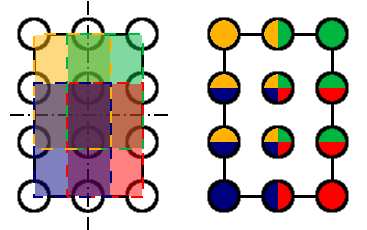
\includegraphics[width=0.4\textwidth]{clusters-automatic}}
          \hspace{0.1\textwidth}
          \subfloat[Задание произвольных областей]{\label{fig:clusters-arbitrary}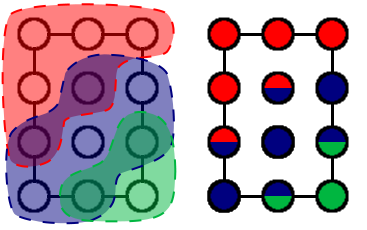
\includegraphics[width=0.4\textwidth]{clusters-arbitrary}}\\
          \caption{Два способа задания кластеров}
          \label{fig:clusters}
        \end{figure}

        Кластеры могут быть заданы двумя способами. В простейшем случае можно выполнить автоматическое
        разбиение объекта плоскостями, перпендикулярными каждой из осей и делящими ось на равные
        отрезки. Для этого в конструктор объекта нужно передать требуемое количество кластеров по
        каждой из осей и степень их перекрытия (в процентах от ширины). Такое разбиение на кластеры
        вполне подходит для однородных объектов простой формы. Если же это не так, можно задать
        кластеры произвольной формы вручную. При этом в конструктор передаётся набор областей в
        пространстве, на основе каждой из которых строится кластер, содержащий все вершины, входящие
        в эту область. Набор областей представляется в виде динамического массива указателей на
        экземпляры класса IRegion, описанного ниже.
        % TODO пояснить иллюстрацию словами

        \paragraph{Внешние воздействия.}
        Информация о~воздействиях может быть сообщена объекту двумя способами. Во-первых,
        функция Model::hit мгновенно изменяет скорость вершин, входящих в~заданную область. Область
        задаётся объектом класса, производного IRegion, в~котором определён метод contains,
        возвращающий true, если данная точка принадлежит области. Другой способ~--- передать в~функцию
        Model::compute\_next\_step, выполняющую вычисление очередного шага алгоритма, массив указателей
        на экземпляры классов-наследников Force, описывающих приложенные к объекту силы. Действие этих
        сил будет учтено при интегрировании скоростей. Для создания собственной реализации силы,
        необходимо в~классе, производном от Force определить метод is\_applied\_to, определяющий,
        приложена ли сила к~вершине, находящейся в данной точке, и метод get\_value\_at,
        возвращающий вектор силы в этой точке.

        \includefigure{core-interaction}{получение информации о внешних воздействиях.}

        \paragraph{Характеристики объекта как целого.}
        Как уже упоминалось в п.~\ref{sssec:proposed_changes} и п.~\ref{sssec:events}, в~процессе
        моделирования возникает необходимость в~определении усреднённых линейной и угловой скоростей
        объекта и рамы и в последующем интегрировании этих скоростей. Первую задачу решает класс
        DiscreteBody, вторую~--- RigidBody. Класс DiscreteBody также отвечает за демпфирование колебаний
        объекта и обеспечение движения рамы как твёрдого тела. Он позволяет привести скорости всех
        входящих в него вершин к вычисленным усреднённым величинам (с~некоторым коэффициентом или в
        точности). В~свою очередь, RigidBody позволяет интегрировать движение, обратное
        к движению жёсткой рамы. Получаемая при этом матрица поворота используется в процессе
        обнаружения отклонения вершины от начальной позиции.

        \includefigure{core-bodies}{расчёт и интегрирование характеристик объекта как целого.}

        \paragraph{Реакции на события.}
        Реакции на три вида поддерживаемых событий: удар в~заданное множество вершин, отклонение от
        начальной формы и вход в~заданную область~--- определяются в~методе invoke класса,
        производного от одного из базовых: соответственно HitReaction, ShapeDeformationReaction или RegionReaction.
        Каждый из этих классов содержит параметры события, которые
        необходимо передать в~его конструктор. Для HitReaction это пороговая абсолютная величина
        изменения скорости вершины при ударе, а также множество вершин, заданное набором индексов вершин
        в~массиве, в котором они были переданы в~конструктор объекта. Параметрами для
        реакции на изменение формы являются множество вершин, заданное аналогичным образом, и минимальное
        отклонение позиции вершины от начальной позиции, при котором событие считается произошедшим.
        RegionReaction хранит в себе указатель на IRegion, также при создании можно указать, что
        является событием: вход в заданную этим указателем область или выход из неё.

        \includefigure{core-reactions}{определение реакции на события.}

        \paragraph{Параллельные вычисления.}
        Как уже говорилось в подразделе~\ref{ssec:parallel}, алгоритм разбивается на задачи, параллельное
        выполнение которых обеспечивается менеджером задач. В~данном случае менеджер задач представляет собой
        потокобезопасную очередь, описанную в п.~\ref{sssec:task_manager}. Различные задачи
        наследуются от базового класса AbstractTask, содержащего чисто виртуальный метод выполнения
        задачи.  Поскольку задача обработки всего объекта должна выполняться после завершения всех
        задач первого этапа, она добавляется в~очередь последней. Кроме того, в её начале
        выполняется ожидание всех событий, устанавливаемых при завершении каждой из задач первого
        этапа, чтобы гарантировать то, что эти задачи уже выполнены, поскольку очередь задач этого не гарантирует.

        Использование каких-либо определённых примитивов синхронизации может ухудшить переносимость
        системы. Необходимо предоставить возможность для замены используемого набора примитивов.
        Это достигается за счёт использования шаблона проектирования <<Абстрактная фабрика>> (\eng{Abstract
        Factory}). Различные примитивы представлены в виде абстрактных классов, а отдельный
        абстрактный класс (<<фабрика>>) содержит методы для создания экземпляров каждого из этих
        классов. Для замены набора примитивов достаточно передать в~систему новую реализацию
        <<фабрики>>.

        \includefigure{parallel}{абстрактная фабрика примитивов синхронизации.}

        Впрочем, необходимо с~осторожностью использовать блокирующие примитивы синхронизации для
        ограничения доступа к разделяемым данным, поскольку их неправильное применение может
        привести к~тому, что задачи, ожидающие доступ к~этим данным, будут выполняться
        последовательно, а не параллельно.  Например, в~данной задаче поправки к скорости вершины от
        разных кластеров усредняются. Если суммировать поправки по мере их вычисления, во время
        выполнения операции суммирования только один поток должен иметь доступ к области памяти,
        в~которой хранится сумма. Остальные потоки, которые также готовы выполнить суммирование,
        будут в~это время простаивать. Чтобы избежать этого, каждый кластер записывает свою поправку
        в~отдельную область памяти, и суммируются они уже после завершения расчётов для кластеров:
        это действие входит в последнюю задачу.

        \paragraph{Использование.}
        Таким образом, типичный сценарий работы с~классом Model следующий. Инициализация:
        \begin{enumerate}
          \item Создание экземпляра: в конструктор передаются исходные массивы физических и
          отображаемых вершин, их описатели (VertexInfo), а также параметры разбиения на кластеры:
          количество и степень перекрытия.
          \item Задание недеформируемой рамы: метод set\_frame.
          \item Определение реакций на события: методы add\_hit\_reaction,\\
          add\_shape\_deformation\_reaction и add\_region\_reaction\\
          (не были показаны на диаграммах для краткости).
        \end{enumerate}
        В теле основного цикла (в случае однопоточного приложения и обновления отображаемой сетки на
        центральном процессоре):
        \begin{enumerate}
          \item Сообщение об ударе: метод hit.
          \item Расчёт шага алгоритма.
          \item Обновление отображаемой сетки.
        \end{enumerate}
        Второй и третий пункт будут подробнее описаны в последующих абзацах

        \paragraph{Расчёт шага алгоритма.}
        В случае однопоточного приложения для расчёта шага алгоритма осуществляется при вызове метода
        compute\_next\_step. В случае многопоточного ~--- при выполнении следующей
        последовательности действий:
        \begin{enumerate}
          \item В главном потоке~--- подготовка очереди задач: метод prepare\_tasks.
          \item В каждом из рабочих потоков~--- выполнение очередной задачи: метод complete\_next\_task.
          \item В главном потоке~--- ожидание окончания расчёта кластеров, после чего можно
            обновлять отображаемую сетку: метод wait\_for\_clusters.
          \item В главном потоке~--- проверка на наличие произошедших событий: метод
            react\_to\_events (производится параллельно выполнению последней задачи рабочим потоком,
            как и обновление отображаемой сетки).
        \end{enumerate}

        \paragraph{Обновление отображаемой сетки.}
        Чтобы выполнить обновление вершин отображаемой сетки на центральном процессоре, необходимо вызвать метод
        update\_vertices, передав ему указатель на массив вершин и описатель вершины.
        Если же используется графический процессор, то вместо этого необходимо
        получить параметры кластеров (матрицы преобразования вершин и нормалей, а также начальный и
        текущий центр масс) с помощью соответствующих методов и передать их в константные регистры
        вершинного шейдера. Важно, что при этом пользователь системы должен выделить в своей структуре,
        представляющей отображаемую вершину, место для хранения массива индексов кластеров и их
        числа. Как было показано в п.~\ref{sssec:using_gpu}, эти данные требуются для расчёта
        позиций отображаемых вершин на графическом процессоре. Пользователь должен также реализовать
        в своём вершинном шейдере вычисление новых позиций вершин и значений связанных с вершинами
        точек и векторов по формулам \eqref{eq:graphical_pos}--\eqref{eq:normal_vectors}.
        Для этого вместе с библиотекой предоставляется фрагмент исходного кода шейдера на языке HLSL,
        выполняющий эти вычисления, так что он может быть вставлен в шейдер, если он также написан
        на HLSL. В противном случае необходимо портировать этот фрагмент на используемый язык.

      \subsubsection{Подсистема математических расчётов}\label{sssec:math}

        Для функционирования основного алгоритма, описанного в подразделе \ref{ssec:basic_algorithm}, требуются
        функции векторной и матричной алгебры. Для этого подсистема математических расчётов содержит
        классы Vector и Matrix, реализующие стандартный набор алгебраических операций. Нетривиальные
        функции описаны ниже.

        \paragraph{Обращение матрицы.}
        Обратная матрица находится как транспонированная матрица алгебраических дополнений, делённая
        на определитель исходной матрицы. Этот метод больше подходит для программной реализации, чем
        метод Гаусса-Жордана, поскольку представляет собой простую формулу, а не итеративный
        алгоритм.

        \paragraph{Диагонализация матрицы.}
        Приведение матрицы к диагональному виду осуществляется методом вращений Якоби (англ.
        \eng{Jacobi rotation})~--- быстрым приближенным итеративным методом \cite{fortran-jacobi}.

        \paragraph{Вычисление функции от матрицы.}
        Для вычисления функции от матрицы она диагонализуется, после чего функция применяется к
        диагональным элементам и матрица преобразуется обратно в исходный базис.

        \paragraph{Полярное разложение.}
        Полярное разложение матрицы $\matx M$ на ортогональную $\matx R$ и симметричную $\matx S$ компоненты
        $\matx M = \matx R \matx S$ осуществляется следующим образом:
        \begin{eqnarray*}
          \matx S & = & \sqrt{\matx{M}^\transposed \matx{M}},\\
          \matx R & = & \matx M \matx{S}^{-1}.
        \end{eqnarray*}
        Здесь используется описанная выше функция вычисления функции от матрицы: в качестве функции
        выступает квадратный корень.

      \subsubsection{Подсистема журналирования и обработки ошибок}
        \includefigure{logging}{структура подсистемы журналирования и обработки ошибок.}

        Основной класс этой подсистемы, Logger, реализует шаблон проектирования <<Одиночка>> (англ.
        \eng{singleton}), что обеспечивает работу с одним и тем же объектом по всей системе без
        необходимости передачи его по всей цепочке вызовов. Чисто виртуальный класс Action
        используется для задания действия, выполняемого в ответ на то или иное событие (запись в
        журнал, предупреждение, ошибка). В подсистеме представлены простейшие реализации действий по
        умолчанию, пользователь же может определить своё действие в~классе, производном от Action. Класс
        Logger содержит следующие методы.
        \begin{enumerate}
          \item Определение действия для конкретного события: метод set\_action.
          \item Отключение реакции на конкретное событие: метод ignore.
          \item Вызов действия: метод invoke.
        \end{enumerate}

    \subsection{Тестирование}

      Корректность работы системы тестируется на двух уровнях: на уровне отдельных функций и на
      уровне системы в~целом. Для тестирования отдельной функции применяется юнит-тестирование:
      пишется несколько тестов, проверяющих корректность её работы в~характерных случаях. Таким
      образом удобно тестировать все функции подсистемы математических расчётов и подсистемы
      журналирования и обработки ошибок, функции доступа к~полям классов, обработку некорректных
      аргументов, расчёт таких предсказуемых величин, как центр масс кластера или
      момент инерции объекта. Преимуществами юнит-тестирования являются лёгкость локализации ошибки
      (за счёт того, что сразу известно, какая функция работает некорректно) и возможность
      убедиться, что система по-прежнему работоспособна после внесения изменений, в~том числе
      после рефакторинга или оптимизации. В~то же время, не менее важно тестировать правдоподобность
      моделируемых деформаций. Но сформулировать математический критерий правдоподобности сложно,
      поэтому юнит-тесты плохо подходят для такого тестирования. Чтобы оно могло осуществляться
      человеком, разработано простое интерактивное приложение, позволяющее пользователю подвергать
      тестовый объект различным воздействиям и наблюдать изменения, происходящие при этом с
      трёхмерной моделью объекта.

  \section{Результаты}\label{sec:results}

    Система моделирования деформаций была реализована в~виде статической
    библиотеки объектных модулей, написанной на языке C++. Было разработано тестовое приложение,
    использующее эту библиотеку, которое средствами API DirectX~9 отображает трёхмерную модель
    объекта и позволяет моделировать его деформации под действием ударов с разных сторон. Трёхмерная
    модель может быть загружена в приложение из файла либо сгенерирована по заданным параметрам при
    запуске.

    В~последующих подразделах описаны результаты экспериментов, выполненных в этом приложении над
    тестовыми объектами, выявленные при этом требования к входным данным и прочие ограничения,
    а~также обнаруженные особенности используемого метода моделирования.

    \subsection{Тестовые объекты}

      Для проверки правдоподобности деформаций и измерения производительности использовались два
      тестовых объекта: <<Цилиндр>> (с~простой геометрией) и <<Автомобиль>> (с~более сложной
      геометрией), они рассмотрены далее. Тестовое приложение запускалось на компьютере со следующими
      характеристиками: четырёхъядерный процессор Intel Core 2 Quad Q6600, тактовая частота 2.4 ГГц,
      видеоадаптер NVIDIA GeForce 8800 GTX.

      \subsubsection{Цилиндр}\label{sssec:cylinder}


        % TODO цифры перепроверить
        В качестве объекта с простой геометрией используется цилиндр, содержащий
        2400 точек в физической модели, сгруппированные в 16 кластеров, и 20000 вершин (13500
        полигонов) в отображаемой сетке. Цилиндр показан на рис.~\ref{fig:cylinder-initial},
        изображение получено в тестовом приложении.

        % TODO определить окружение для этого
        \begin{figure}[!htb]
          \centering
          \subfloat[Исходное состояние]{\label{fig:cylinder-initial}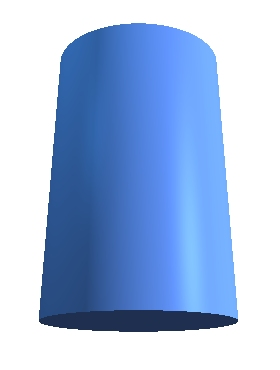
\includegraphics[width=0.3\textwidth]{cylinder}}
          \subfloat[Удар в середину]{\label{fig:cylinder-deformed-1}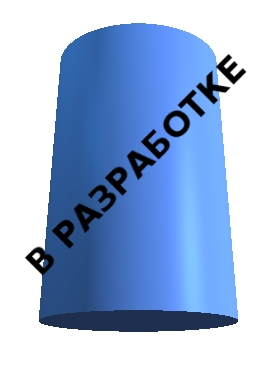
\includegraphics[width=0.3\textwidth]{cylinder-deformed-1}}\\
          \subfloat[Удар в край]{\label{fig:cylinder-deformed-2}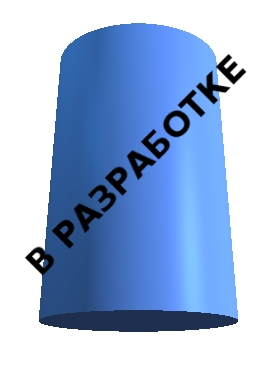
\includegraphics[width=0.3\textwidth]{cylinder-deformed-2}}
          \subfloat[Комбинация ударов]{\label{fig:cylinder-deformed-3}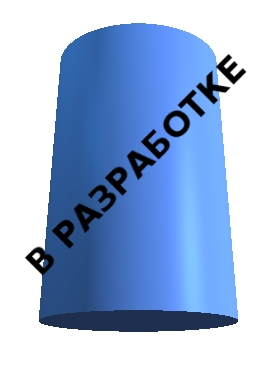
\includegraphics[width=0.3\textwidth]{cylinder-deformed-3}}
          \caption{Тестовый объект <<Цилиндр>>}
          \label{fig:cylinder}
        \end{figure}

        Были протестированы следующие случаи воздействия на объект.
        \begin{enumerate}
          \item Поперечный удар в середину объекта, см. рис.~\ref{fig:cylinder-deformed-1}.
          \item Продольный удар в край объекта, см. рис.~\ref{fig:cylinder-deformed-2}.
          \item Комбинация ударов, см. рис.~\ref{fig:cylinder-deformed-3}.
        \end{enumerate}

        \note{настоящие картинки ещё не получены, но будут получены в ближайшее время.}

        Также было проведено исследование зависимости времени расчётов от числа вершин в физической
        модели и отображаемой сетке. Для каждого числа вершин производилось 5 запусков тестового
        приложения, каждый из которых длился 1 минуту. На объект оказывались одинаковые воздействия. Во время
        исполнения на каждом кадре измерялось время, требуемое для физического моделирования и для
        вычисления позиций вершин отображаемой сетки. По получаемой выборке рассчитывалось
        % TODO больше думать про обработку данных
        среднее значение. Многократные запуски необходимы, чтобы исключить
        факторы, внешние по отношению к~приложению, например, загрузку процессора другими приложениями
        и операционной системой. Результаты измерений представлены в виде графика на рис.~\ref{fig:time-plot}.

        \includefigure[width=1\linewidth]{time-plot}{зависимость времени вычисления от числа физических и отображаемых вершин.}

        % TODO сравнение CPU/GPU TODO <- вспомнить что я хотел этим сказать
        \paragraph{Выводы.} Зависимость от числа вершин обоих типов близка к линейной.
        Горизонтальный участок зависимости для отображаемых вершин связан с тем, что, даже когда
        вычисления на графическом процессоре занимают очень мало времени, имеются
        постоянные накладные расходы времени. Например, на передачу данных между графическим и центральным
        процессором и на растеризацию изображения. Из графика следует, что затраты времени на
        одну вершину физической модели значительно выше затрат на одну отображаемую вершину. Таким
        образом, использование физической модели с~меньшим числом вершин и последующее отображение
        её деформаций на отображаемую сетку с~б\'{о}льшим числом вершин оправдано.

      \subsubsection{Автомобиль}

        % TODO цифры перепроверить
        В качестве объекта со сложной геометрией используется автомобиль, содержащий
        2800 точек в физической модели, сгруппированные в~32 кластера, и 28000 вершин (67500
        полигонов) в отображаемой сетке. Исходная форма объекта показана на рис.~\ref{fig:car-initial}.

        % TODO определить окружение для этого
        \begin{figure}[!htb]
          \centering
          \subfloat[Исходное состояние]{\label{fig:car-initial}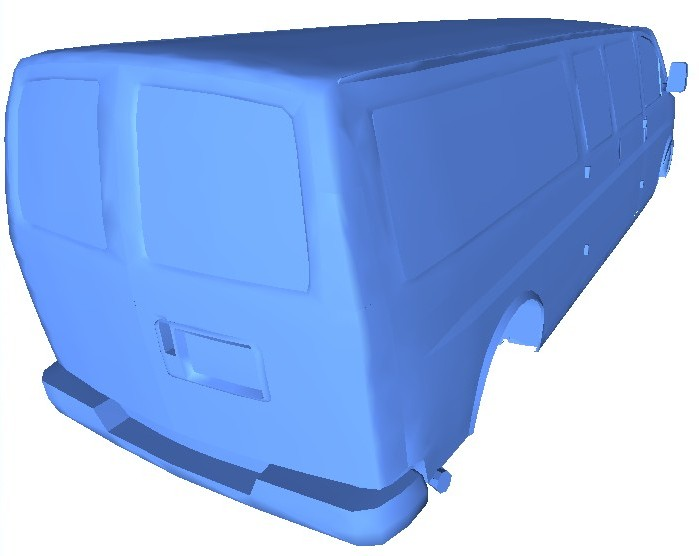
\includegraphics[width=0.4\textwidth]{car}}
          \subfloat[Удар в середину]{\label{fig:car-deformed-1}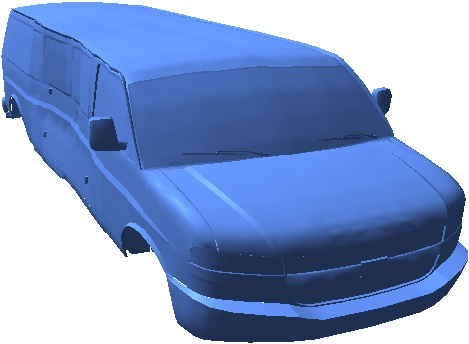
\includegraphics[width=0.4\textwidth]{car-deformed-1}}\\
          \subfloat[Удар в край]{\label{fig:car-deformed-2}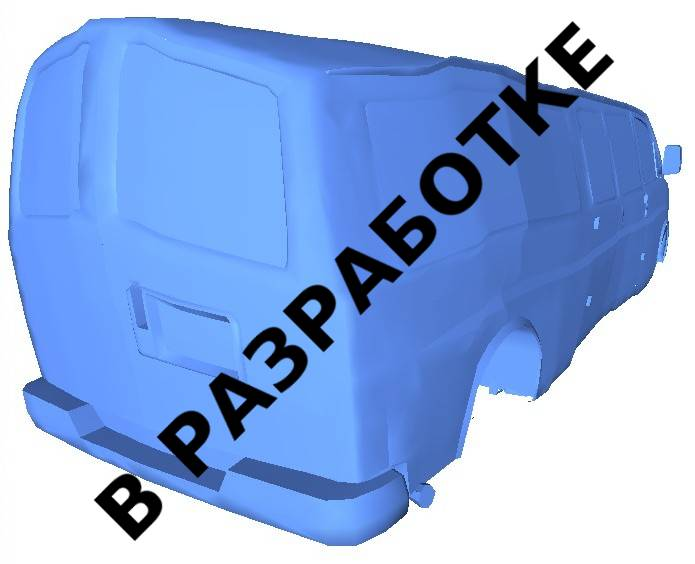
\includegraphics[width=0.4\textwidth]{car-deformed-2}}
          \subfloat[Комбинация ударов]{\label{fig:car-deformed-3}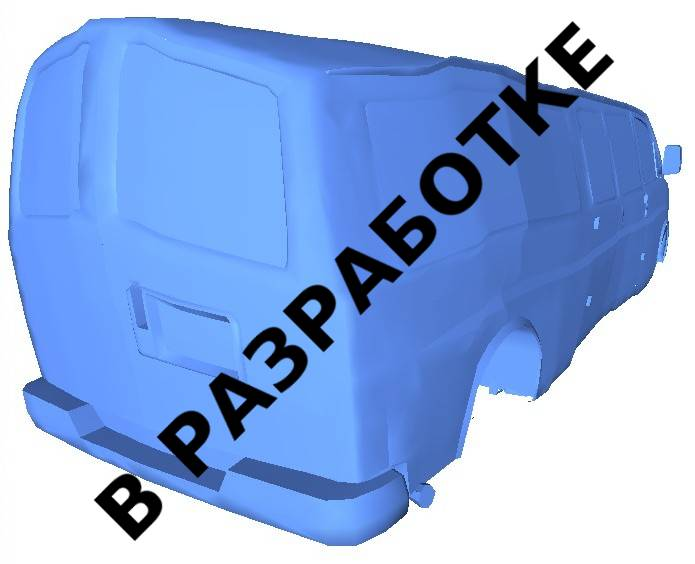
\includegraphics[width=0.4\textwidth]{car-deformed-3}}
          \caption{Тестовый объект <<Автомобиль>>}
          \label{fig:car}
        \end{figure}

        Были протестированы следующие случаи воздействия на объект.
        \begin{enumerate}
          \item Поперечный удар в середину объекта, см. рис.~\ref{fig:car-deformed-1}.
          \item Продольный удар в край объекта, см. рис.~\ref{fig:car-deformed-2}.
          \item Комбинация ударов, см. рис.~\ref{fig:car-deformed-3}.
        \end{enumerate}

        \note{настоящие картинки ещё не получены, но будут получены в ближайшее время.}

        % TODO как гарантировать распределение по ядрам?
        Чтобы проверить масштабируемость многопоточного алгоритма, сравнивалось быстродействие
        версий тестового приложения с разным числом рабочих потоков, от 1 до 4, на четырёхъядерном
        процессоре. Как было показано в п.~\ref{sssec:parallel_tasks}, вычисления разбиваются на два
        этапа, и только задачи первого этапа независимы и выполняются параллельно, а остальные
        вычисления производятся после завершения первого этапа. Поэтому измерялось отдельно время,
        требуемое для каждого этапа. Ожидалось, что для первого этапа оно будет убывать обратно
        пропорционально числу потоков, а для второго этапа~--- оставаться неизменным. Реально
        полученные результаты представлены на рис.~\ref{fig:thread-plots}: диаграмма на
        рис.~\ref{fig:time-plot-threads} показывает зависимость времени расчётов от числа потоков, а
        график на рис.~\ref{fig:speedup-plot}~--- выраженное в процентах отношение затрат времени
        однопоточной версией к затратам при данном числе потоков, показывающее, во сколько раз
        многопоточная версия системы быстрее однопоточной.

        % TODO определить окружение для этого
        \begin{figure}[!htb]
          \centering
          \subfloat[Время вычислений]{\label{fig:time-plot-threads}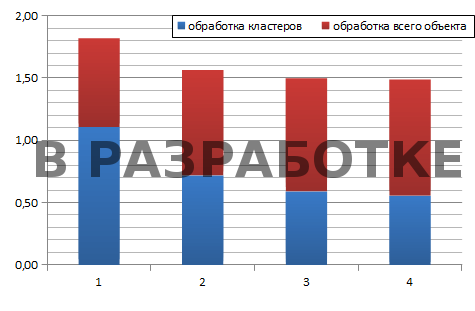
\includegraphics[width=0.5\textwidth]{time-plot-threads}}
          \subfloat[Относительное ускорение]{\label{fig:speedup-plot}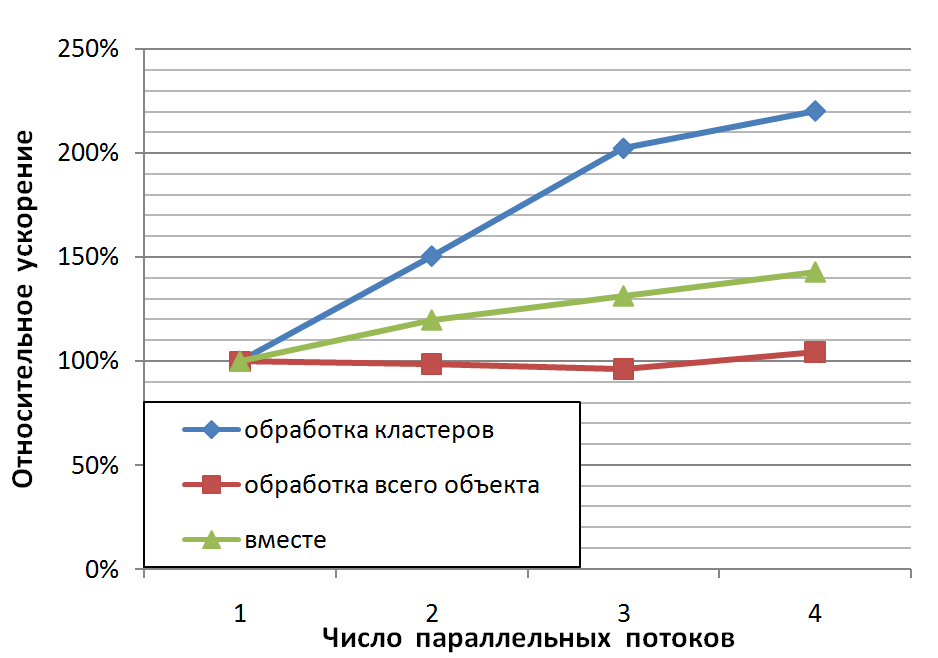
\includegraphics[width=0.5\textwidth]{speedup-plot}}
          \caption{Зависимость скорости вычислений от числа потоков, выполняющихся на разных ядрах процессора}
          \label{fig:thread-plots}
        \end{figure}

        \paragraph{Выводы.}
        Наблюдается рост скорости вычислений, выполняемых параллельно, при увеличении числа потоков.
        Характер этого роста далёк от линейного, но при одновременной работе всех четырёх
        ядер процессора достигается ускорение в два раза. Тем не менее, задача обработки всего
        объекта в многопоточной версии библиотеки выполняется дольше, из-за чего суммарное время
        расчётов при нескольких потоках оказывается лишь незначительно меньше, чем в однопоточной
        версии.
        \note{зависимость от числа потоков и вывод пока предварительные. Есть надежда, что конечные
        результаты будут значительно лучше.}

    \subsection{Оптимальные значения параметров}\label{ssec:optimal_parameters}

      Параметрами представления объекта являются распределение плотности точек и массы в
      пространстве, форма и число кластеров, размер и положение недеформируемых частей, а также
      численный параметр~--- коэффициент затухания колебаний. Каждый кластер имеет свой набор
      параметров, влияющих на моделирование неупругости: порог деформации, при которой начинает
      проявляться неупругость, скорость изменения формы при этом, а также максимальная величина
      остаточной деформации. \todo{Сказать, в каких попугаях это всё меряется.} Были определены
      допустимые интервалы этих параметров, их физический смысл и влияние их на характер
      моделируемых деформаций.

      % TODO говорить ли про beta из T = (1-b)A + bR, если я в это не углублялся в теории?

      \note{Эти результаты ещё не готовы, хотя определённые закономерности были замечены и учтены в
      процессе разработки.}

      % Оптимальное число кластеров было определено экспериментальным
      % путём для достижения компромисса между детальностью моделируемых деформаций и быстродействием.
      % TODO Обоснование поподробнее.

      % TODO Ещё что-то сказать насчёт того, во сколько кластеров может входить одна вершина, сюда
      % идёт ссылка из реализации и из ограничений (полагается 8).

    \subsection{Требования к входным данным}\label{ssec:requirements}

      \paragraph{Требования к представлению объекта}
      Жёсткость конкретной области поверхности объекта существенно зависит от плотности точек в этой
      области. Во-первых, если между соседними точками имеется значительный промежуток, то изгиб
      объекта в~этом промежутке не может быть смоделирован из-за отсутствия в~нём точек. Во-вторых,
      проблема возникает, если значительная по объёму часть кластера содержит намного меньше точек,
      чем остальная часть кластера. Тогда при подборе формы вклад этого небольшого числа точек будет
      также незначителен, и, несмотря на сильное отклонение в этой области, деформация всего
      кластера может оказаться слабой. Таким образом, чтобы моделирование было реалистичным,
      фрагменты модели, состоящие из однородного материала, должны представляться набором точек
      равномерной плотности.

      \paragraph{Требования к разбиению на кластеры}
      Используемый метод подбора формы накладывает ограничение на исходную форму, образуемую
      вершинами одного кластера. При подборе формы вычисляется оптимальное линейное преобразование
      множества точек, входящих в кластер, переводящее его из исходного состояния в наиболее близкое
      к текущему. Это преобразование будет неоднозначным, если множество точек лежит в одной
      плоскости или на одной прямой, будь то в исходном или текущем состоянии. Если такую форму
      имеет текущее состояние кластера, подбор формы на этом шаге может быть пропущен, а значений
      целевых позиций могут быть взяты с прошлого шага. Если же проблема заключается в
      исходной форме, подбор формы не сможет быть выполнен ни на одном шаге, поэтому система сообщит
      об ошибке при попытке создания объекта, содержащего хотя бы один такой некорректный кластер.
      В этом случае нужно либо изменить разбиение на кластеры, либо добавить в некорректный кластер
      дополнительные точки, например, разделив плоскость на два близких слоя с~массой, равной
      половине исходной массы.

    \subsection{Ограничения}\label{sssec:limitations}

      Реализация системы не имеет принципиальных ограничений на количество вершин, кластеров и других сущностей,
      используемых при моделировании, поскольку они хранятся в массивах динамически изменяемого размера.
      Тем не менее, в~зависимости от характеристик компьютера, на котором используется система, при слишком
      больших значениях ресурсы этого компьютера могут быть исчерпаны, либо быстродействие системы
      может оказаться ниже требуемого. Эти случаи рассмотрены в последующих пунктах данного
      подраздела.

      Кроме того, ограниченно максимальное число кластеров, в которое может входить одна физическая
      или отображаемая вершина, что было объяснено в п.~\ref{sssec:impl_core}.

      \subsubsection{Скорость расчёта}

        % TODO сказать там про цифры
        Как уже говорилось в разделе~\ref{sec:task}, расчёт одного кадра в приложении виртуальной реальности должен
        занимать не более 33~мс, из которых на расчёт деформаций отводится обычно около 3--5 мс. Рис.~\ref{fig:time-plot}
        из п.~\ref{sssec:cylinder} показывает пример роста времени расчётов от основных параметров,
        влияющих на быстродействие: числа физических и отображаемых вершин в представлении объекта.
        Таким образом, для достижения требуемого времени расчётов можно манипулировать обоими
        параметрами. Причём, поскольку в случае физических вершин рост намного быстрее, значительное
        уменьшение их числа является хорошим способом повышения быстродействия без уменьшения
        детализации отображаемой модели объекта. Однако качество моделирования деформаций при этом
        может снизиться.

      \subsubsection{Объём используемой оперативной памяти}

        Наибольший объём памяти в системе требуется для хранения физических и отображаемых вершин в
        силу их большого числа. Размер структур, представляющих каждый видов вершин, зависит от
        максимального числа кластеров, в которое может входить вершина, поскольку, как было показано
        в п.~\ref{sssec:impl_core}, каждая из вершин хранит статический массив соответствующего
        размера. Далее предполагается, что это число равно 8, оптимальному в большинстве случаев
        согласно рассуждениям в подразделе~\ref{ssec:optimal_parameters}.

        % TODO перепроверить цифры, подумать об оптимизации
        Структура, представляющая физическую вершину занимает в памяти 312 байт. Например, если
        физическое представление объекта должно занимать не более 10 мегабайт, то максимальное
        возможное число вершин в этом представлении~--- 32 051. Как уже было сказано выше, это не
        является серьёзным ограничением, поскольку число физических вершин может быть уменьшено без
        влияния на детализацию отображаемого объекта.

        Затраты памяти на хранение информации об отображаемых вершинах зависят от способа вычисления
        их позиций. Если оно выполняется на графическом процессоре, то информация об отображаемых
        вершинах не требуется в~процессе моделирования, и используется только при создании объекта.
        При этом нужно 48 байт на каждую вершину, причём эта память будет освобождена после
        завершения инициализации объекта. Кроме этого, как уже говорилось в п.~\ref{sssec:impl_core},
        в структуре, используемой в приложении для представления отображаемой вершины, пользователь
        должен выделить место для хранения 8 индексов и их числа.  Если число кластеров не больше
        255 (что является разумным ограничением, как было показано в подразделе~\ref{ssec:optimal_parameters}),
        то для хранения индексов и их числа можно использовать 1 байт. Таким образом,
        размер пользовательской структуры увеличивается на 9 байт при использовании вычислений на
        графическом процессоре. Это нужно учитывать, если объём используемой в приложении
        оперативной памяти или памяти видеоадаптера высок и увеличение может привести к проблемам.

        Если же обновление отображаемой сетки выполняется на центральном процессоре, необходимо
        сохранять информацию о всех связанных с отображаемой вершиной векторах и точках, а~также об
        ортогональности каждого вектора (необходимость этой информации была объяснена подробнее в
        п.~\ref{sssec:using_gpu}). Допустим, с каждой отображаемой вершиной может быть связано
        не более 5 векторов и 5 точек, тогда размер структуры, представляющей эту вершину в~системе,
        составит 280 байт. Если стоит требование, что максимальное количество памяти, расходуемой на
        графическое представление объекта равно, например, 10 мегабайтам, то число вершин не может
        быть больше 35 714. Этого может быть недостаточно для отображения объекта со сложной
        геометрией, поэтому, в отличие от физических вершин, недостаток памяти для хранения
        отображаемых вершин может быть серьёзной проблемой, если обновление их позиций выполняется
        на центральном процессоре.

      \subsubsection{Ограничения графического процессора}

        Число константных регистров вершинного шейдера ограничено. В п.~\ref{sssec:using_gpu} было
        показано, что на каждый кластер требуется 7 таких регистров. Таким образом, число регистров
        вершинного шейдера накладывает ограничение на максимальное возможное число кластеров в
        представлении объекта.

        Например, в графических адаптерах, которые поддерживают спецификацию \eng{Shader Model~4},
        гарантируется наличие 65536 таких регистров. Максимальное возможное число
        кластеров при этом равно $\lfloor 65536/7 \rfloor = 9362$. Как было показано
        в~разделе~\ref{sec:results}, это значительно больше оптимального числа кластеров для
        типичного моделируемого объекта. Таким образом, при использовании \eng{Shader Model~4}
        количество регистров не накладывает существенного ограничения на число кластеров. Однако
        версии DirectX 10 и 11, поддерживающие \eng{Shader Model~4}, ещё недостаточно широко
        распространены \cite{steam-hardware}.

        Если же видеоадаптер поддерживает только менее современную спецификацию \eng{Shader
        Model~3}, то гарантированно он имеет только 256 константных регистров вершинного шейдера.
        Поэтому максимальное теоретически возможное число кластеров~--- это $\lfloor 256/7 \rfloor = 36$.
        В~реальности оно ещё меньше, поскольку часть регистров требуется приложению для
        расчётов, связанных с~получением изображения. При использовании данной системы в~режиме
        вычислений на графическом процессоре её пользователь должен учитывать это ограничение и,
        если оно является неприемлемым, использовать режим вычислений на центральном процессоре.

    \subsection{Особенности используемого метода}

        Поскольку основной алгоритм является геометрическим, при определённых условиях моделирование
        может быть нереалистичным. Далее описаны некоторые характерные свойства этого алгоритма и их
        влияние на реалистичность деформаций.

        \paragraph{Свойства области пересечения кластеров.} Было обнаружено, что удар в область,
        принадлежащую только одному кластеру, и удар в область пересечения кластеров оказывают
        различное влияние на объект. А именно, во втором случае область распространения деформаций
        оказывается больше из-за того, что большее число кластеров изменяет свою форму. Это свойство
        может быть использовано, чтобы моделировать ребро жёсткости областью пересечения соседних
        % TODO подумать, насколько это реально
        кластеров: её собственная форма будет изменяться слабо (поскольку входящие в неё кластеры
        будут примерно одинаково изменять свою форму), но при этом удар непосредственно в неё будет
        оказывать большое влияние на соприкасающиеся кластеры. Если же это не требуется, такое
        свойство может быть нежелательным побочным эффектом. В дальнейшем планируется предусмотреть
        возможность ограничения области распространения удара, чтобы исключить эту проблему.

        \paragraph{Невозможность сложных деформаций отдельного кластера.} В связи с тем, что для сохранения
        деформируемого состояния каждого кластера используется матрица $3 \times 3$, задающая
        линейное преобразование, множество возможных деформаций отдельного кластера ограничено комбинациями
        поворотов, сжатий и продольных сдвигов. Это может быть полезным, если не требуется
        моделировать изгиб частей объекта, задаваемых кластерами. Но в большинстве случаев это не
        так, поэтому требуется учащение разбиения на кластеры в местах, где моделирование
        изгибов необходимо. Оптимальное число кластеров в подразделе~\ref{ssec:optimal_parameters}
        определялось с учётом этого факта.

  \section{Дальнейшая работа}

    В дальнейшем планируется работа по ослаблению требований, перечисленных
    в подразделе~\ref{ssec:requirements}. В~частности, описанные там же действия для коррекции
    представления объекта и разбиения на кластеры могут выполняться автоматически.

    Алгоритм имеет довольно много входных параметров, включая разбиение на кластеры и
    различные численные параметры, описанные в подразделе~\ref{ssec:optimal_parameters}. Задание их вручную в коде для каждого
    объекта является неудобным. Планируется разработка программного модуля для редактора
    трёхмерной графики Autodesk 3ds Max, в котором дизайнер сможет удобным способом задавать эти параметры. При этом
    будет разработан собственный формата файла для хранения этих параметров, разбор которого будет
    осуществляться внутри данной системы. Это позволит применять систему в~реальных приложениях
    виртуальной реальности, которые обычно содержат множество разнообразных деформируемых объектов.

  \section{Заключение}\label{sec:conclusion}

    В данной работе ставилась цель разработать систему моделирования деформаций неупругих тел
    в~реальном времени, ориентированную на применение в~приложениях виртуальной реальности. Эта цель
    была достигнута, и были удовлетворены поставленные в разделе~\ref{sec:task} требования, включая
    высокое быстродействие и удобный для интеграции интерфейс, а~также применение параллельных
    вычислений и отказ от использования предварительно рассчитанных деформаций. Предусмотрено
    тестирование системы с~помощью модульных тестов. Также было разработано простое интерактивное
    приложение, использующее возможности системы, чтобы моделировать деформаций предварительно
    заданного объекта. С помощью этого приложения была протестирована правдоподобность деформаций и
    исследованы быстродействие и зависимость характера деформаций от параметров алгоритма. В
    дальнейшем система будет доработана и улучшена. Кроме того, планируется разработка
    дополнительных инструментов, упрощающих использование системы разработчиками приложений
    виртуальной реальности.

  \section{План-график}

    \begin{center}
      \begin{tabular}{|p{10.3cm}|c|c|}\hline
        Задача                                       & Время         & Срок  \\\hline\hline
        Проработка архитектуры системы, разработка и реализация алгоритма деформаций
        с юнит-тестами для тестирования базовых функций и простым тестовым приложением
        для комплексного тестирования                & (выполнено)   & 31.10 \\\hline
        Обнаружение событий и реакция на них         & (выполнено)   & 15.12 \\\hline
        Реализация отображения низкополигональной
        модели на высокополигональную сетку          & (выполнено)   & 15.01 \\\hline
        Разработка интерактивного приложения для
        тестирования правдоподобности деформаций     & (выполнено)   & 15.01 \\\hline
        Профилирование и оптимизация алгоритма       & (выполнено)   & 15.03 \\\hline
        Адаптация алгоритма для параллельных
        вычислений                                   & (выполнено)   & 1.04 \\\hline
      \end{tabular}
    \end{center}

  \section{Оценки за отчёт}

    Руководитель: \underscore{1cm} (из 10). Подпись: \underscore{3cm} (Д.\,А.\,Гладкий)

    \vspace{0.5cm}
    Преподаватель: \underscore{2cm}

  \begin{flushleft}
    \bibliography{../../biblio/my}
  \end{flushleft}
\end{document}

